\documentclass[12pt,a4paper]{article}
\usepackage[utf8]{inputenc}
\usepackage[english]{babel}
\usepackage{amsmath}
\usepackage{amsfonts}
\usepackage{amssymb}
\usepackage{makeidx}
\usepackage{graphicx}
\usepackage{lmodern}
\usepackage{kpfonts}
\usepackage{apacite}
\usepackage{multirow}
\usepackage{graphicx}
\usepackage{framed}
\setlength{\parindent}{0em}
\usepackage[left=3cm,right=3cm,top=2cm,bottom=2cm]{geometry}
\author{Gareth James, Daniela Witten, Trevor Hastie \& Robert Tibshirani}
\title{An Introduction to Statistical Learning\\
\large{(Summary by \textit{Pablo Vivas})}}
\date{January 13, 2020}
\begin{document}
\maketitle
\section{Introduction}
Statistical learning refers to a vast set of tools for \textbf{understanding data}. These tools can be classified as:
\begin{itemize}
\item supervised 
\item unsupervised
\end{itemize}
Broadly speaking, supervised statistical learning involves building a statistical model for predicting, or estimating, an output based on one or more inputs. Problems of this nature occur in fields as diverse as business, medicine, astrophysics, and public policy. With unsupervised statistical learning, there are inputs but no supervising output; nevertheless we can learn relationships and structure from such data.
The datasets used in this books are:
\begin{itemize}
\item Wage 
\item Stock Market
\item Gene Expression
\end{itemize}

\textbf{\textit{Some history}}
\begin{framed}
Legendre and Gauss published papers on the method of \textit{least squares}.\\
Fisher proposed \textit{linear discriminant analysis} in 1936.\\
In the 1940s, various authors put forth an alternative approach, \textit{logistic regression}.\\
In the early 1970s, Nelder and Wedderburn coined the term \textit{generalized linear models} for an entire class of statistical learning methods that include both linear and logistic regression as special cases.\\ 
In mid 1980s Breiman, Friedman, Olshen and Stone introduced \textit{classification and regression trees}.\\
Hastie and Tibshirani coined the term \textit{generalized additive models} in 1986 for a class of non-linear extensions to generalized linear models. 
\end{framed}
\section{Statistical Learning}
Suppose that we observe a quantitative response $Y$ and $p$ different predictors, $X_{1},X_{2},...,X_{p}$. \textbf{We assume} that there is some relationship between $Y$ and $X =(X_{1},X_{2},...,X_{p})$, which can be written in the very general form:
\begin{center}
\boxed{Y = f(X) + \epsilon}
\end{center}
Here $f$ is some fixed but unknown function of $X_{1},X_{2},...,X_{p}$, and $\epsilon$ is a random error term, which is independent of $X$ and has mean zero. In this formulation, $f$ represents the systematic information that $X$ provides about $Y$.\\
\newline
\textit{Why Estimate $f$?}
\begin{itemize}
\item \textit{Prediction}: In many situations, a set of inputs $X$ are readily available, but the output $Y$ cannot be easily obtained. Since the error term averages to zero, we can predict $Y$ using
\begin{center}
 \boxed{\hat{Y}=\hat{f}(X)}
\end{center}
Where $\hat{f}$ represents our estimate for f, and $\hat{Y}$ represents the resulting prediction for $Y$ . \textbf{In this setting,$\hat{f}$ is often treated as a black box}, in the sense that one is not typically concerned with the exact form of $\hat{f}$, provided that it yields accurate predictions for $Y$.\\
\newline
The accuracy of $\hat{Y}$ as a prediction for Y depends on two quantities, which we call the \textit{reducible error} and the \textit{irreducible error}.$\hat{f}$ will not be a perfect estimate for f, and this inaccuracy will introduce some error. This error is reducible because we can potentially improve the accuracy of $\hat{f}$ by using the most appropriate statistical learning technique to estimate f. However, even if it were possible to form a perfect estimate for f, so that our estimated response took the form $\hat{Y}=f(x)$, our prediction would still have some error in it! This is because Y is also a function of $\epsilon$, which, by definition, cannot be predicted using X. Therefore, variability associated with $\epsilon$ also affects the accuracy of our predictions. This is known as the irreducible error, because no matter how well we estimate f, we cannot reduce the error introduced by $\epsilon$.

\item \textit{Inference}: We are often interested in understanding the way that Y is affected as $X_{1},X_{2},...,X_{p}$ change. In this situation we wish to estimate $f$, but our goal is not necessarily to make predictions for Y . We instead want to understand the relationship between X and Y, or more specifically, to understand how Y changes as a function of $X_{1},X_{2},...,X_{p}$. \textbf{Now $\hat{f}$ cannot be treated as a black box}, because we need to know its exact form. In this setting, one may be interested in answering the following questions:
\begin{itemize}
\item Which predictors are associated with the response? 
\item What is the relationship between the response and each predictor? 
\item Can the relationship between Y and each predictor be adequately summarized using a linear equation, or is the relationship more complicated?
\end{itemize}
\end{itemize}
\newpage
\textit{How Do We Estimate $f$?}
\begin{itemize}
\item \textit{Parametric Models}: Parametric methods involve a two-step model-based approach. 
\begin{enumerate}
\item First, we make an assumption about the functional form, or shape, of f. For example, one very simple assumption is that f is linear in X: 
\begin{center}
\boxed{f(X)=\beta_{0}+\beta_{1}X_{1}+\beta_{2}X_{2},...,\beta_{p}X_{p}}
\end{center}
This is a \textit{linear model}. Once we have assumed that f is linear, the problem of estimating f is greatly simplified. Instead of having to estimate an entirely arbitrary p-dimensional function f(X), one only needs to estimate the $p+1$ coefficients $\beta_{0},\beta_{1},..,\beta_{p}$.
\item After a model has been selected, we need a procedure that uses the training data to fit or train the model. In the case of the linear model, we need to estimate the parameters $\beta_{0},\beta_{1},..,\beta_{p}$.  That is, we want to find values of these parameters such that
\begin{center}
$Y \approx \beta_{0}+\beta_{1}X_{1}+\beta_{2}X_{2},...,\beta_{p}X_{p}$
\end{center}
\end{enumerate}

This approach reduces the problem of estimating f down to one of estimating a set of parameters.  Assuming a parametric form for f simplifies the problem of estimating f because it is generally much easier to estimate a set of parameters than it is to fit an entirely arbitrary function f.  The potential disadvantage of a parametric approach is that the model we choose will usually not match the true unknown form of f. If the chosen model is too far from the true f, then our estimate will be poor. We can try to address this problem by choosing flexible models that can fit many different possible functional forms for f. But in general, fitting a more flexible model requires estimating a greater number of parameters. These more complex models can lead to a phenomenon known as overfitting the data, which essentially means they follow the errors, or noise, too closely.

\item \textit{Non-Parametric Models}: Non-parametric methods do not make explicit assumptions about the functional form of f. Instead they seek an estimate of f that gets as close to the data points as possible without being too rough or wiggly. Such approaches can have a major advantage over parametric approaches: by avoiding the assumption of a particular functional form for f, they have the potential to accurately fit a wider range of possible shapes for f. Any parametric approach brings with it the possibility that the functional form used to estimate f is very different from the true f, in which case the resulting model will not fit the data well. In contrast, non-parametric approaches completely avoid this danger, since essentially no assumption about the form of f is made. But non-parametric approaches do suffer from a major disadvantage: since they do not reduce the problem of estimating f to a small number of parameters, a very large number of observations (far more than is typically needed for a parametric approach) is required in order to obtain an accurate estimate for f.
\end{itemize}
\newpage
\textit{Prediction Accuracy and Model Interpretability: The Trade-Off}
\begin{figure}[hbtp]
\centering
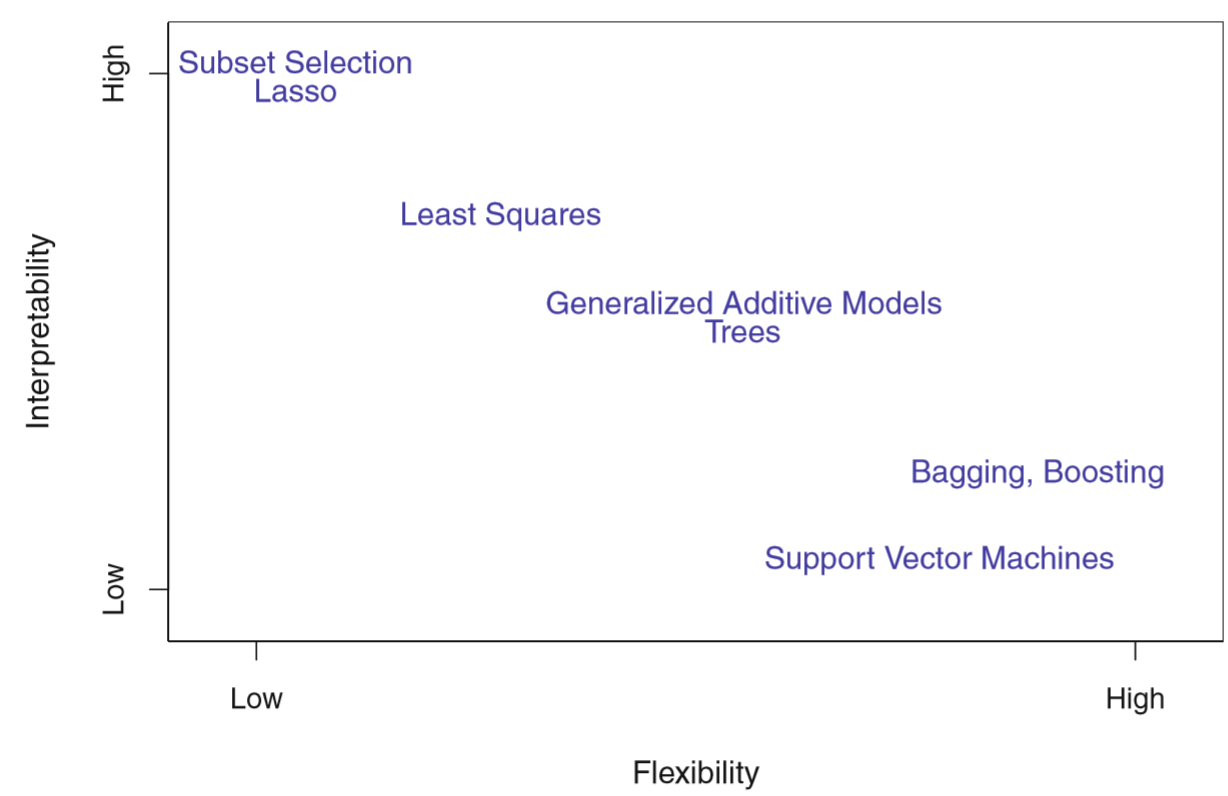
\includegraphics[scale=0.5]{F1.png}
\caption{A representation of the tradeoff between flexibility and interpretability, using different statistical learning methods}
\end{figure}

\section{Linear Regression}
\section{Classification}
\section{Resampling Methods}
\section{Linear Model Selection and Regularization}
\section{Moving Beyond Linearity}
\section{Tree-Based Methods}
\section{Support Vector Machines}
\section{Unsupervised Learning}
\end{document}


